\section{Introduction}
\label{sec:intro}

\subsection{Avant propos}

% On peut distinguer les mathématiques financières en deux classe : le côté vente et le côté
% achat. Le côté vente cherche à déterminer le juste prix d'un instrument lui permettant de
% répliquer les profits et pertes découlant de la vente de cet instrument. Le côté achat
% cherche à établir un portefeuille spéculatif dont l'objectif est de maximiser le rendement
% et d'en diminuer le risque.

% Historiquement, le côté vente a été propulsé par la mise en place de modèles mathématiques
% reposant sur deux hypothèses : l'absence d'arbitrage et le processus stochastique
% modélisant les rendements du sous jacent à l'instrument. Si une de ces deux hypothèses
% s'avère fausse, alors le prix qui aura été déterminé sera à son tour inexact et le vendeur
% sera susceptible de 

% L'objet de ce mémoire est l'étude d'une nouvelle 

% Essentiellement, un investisseur n'a qu'un seul objectif: maximiser ses rendements et
% diminuer ses risques. Par exemple, une institution pourrait être tentée d'investir une
% partie de sa richesse dans l'achat ou la vente à découvert de droits de propriétés (ou
% actions) d'une firme. La décision prise se fera par exemple suite à une analyse
% fondamentale (comptable) qui déterminera la valeur intrinsèque de l'action. Si l'analyste
% juge que la valeur intrinsèque est inférieure au prix affiché sur les marchés boursiers,
% alors achat il y aura. Par contre, une telle analyse ne tient pas forcément compte des
% risques associés à la décision

% Dans les années 1990, le monde de la finance à vu apparaître une nouvelle façon de faire,
% inédite jusqu'alors. En posant deux hypothèses, une institution était soudainement en
% mesure de déterminer la valeur exact d'une option sur un titre financier et d'autre part
% de déterminer un mécanisme de couverture permettant de répliquer les profits et pertes de
% la vente de cette option. Des institutions ont ainsi pu réaliser d'énormes profits  titre.  tout en s'assurant une couverture sur
% les profits et pertes de ce sous-jacent.

% L'objet de ce mémoire est d'introduire un algorithme de gestion de portefeuille à un actif
% inspiré des méthodes d'apprentissage machine modernes. Plusieurs caractéristiques viennent
% distinguer cet algorithme des méthodes classiques d'optimisation de portefeuille: en
% premier lieu, on fera l'hypothèse d'une \textit{loi de marché} probabiliste et multivariée
% dont les réalisations représentent 

% Les \textit{mathématiques financières} telles qu'elles sont professées de nos jours
% reposent sur le simple principe d'absence d'arbitrage. Ainsi, une institution financière
% peut, à l'aide d'arguments issus du calcul stochastique, \textit{tarifer} une option
% vendue à un client en s'assurant d'autre part une \textit{couverture de risque} qui
% balance les profits et pertes. Ainsi, en vendant une option un peu plus chère que son prix
% mathématique cette institution peut elle garantir un revenu sans risque. Une hypothèse
% doit alors cependant être posée, celle de la distribution du processus stochastique
% modélisant les rendements du sous-jacent de l'option.

% Ce mémoire aborde les choses différement. Un modèle sera proposé

Ce mémoire aborde les choses différement. Il n'est plus question de \textit{tarifer} un
instrument financier par hypothèse d'absence d'arbitrage, mais plutôt de déterminer dans
quelle mesure un investissement devrait être considéré en supposant la présence
d'arbitrage dans le marché. La différence est ici 

D'autre part, la théorie moderne de portefeuille, introduite par Markowitz, 

\todo{Discuter du rôle croissant que jouent l'informatique et les statistiques dans la
  construction de portefeuille. Contraster avec les math. stochastiques. Citer Simons et
  cet article de Quandl selon lequel data is the new shit.}


\subsection{Exposition du problème et hypothèses}

Ce mémoire vise donc à établir clairement et rigoureusement comment un investisseur averse
au risque disposant \textit{d'information complémentaire} au \textit{marché} peut utiliser
cette information pour accroître son \textit{utilité espérée} ou, de façon équivalente,
son \textit{rendement équivalent certain}.

\subsubsection{Modélisation du marché}

Nous entendrons ici par \textit{marché} n'importe quel type d'actif financier ou
spéculatif dans lequel on peut investir une partie de sa fortune dans l'espoir de la voir
fructifier au cours d'une période de temps arbitraire. Ainsi, tout au long de l'exposé
théorique qui suivra, il peut être pertinent d'avoir en tête les rendements quotidiens
issus des grands indices boursiers (par exemple les 500 plus grandes capitalisations
américaines). Cependant, le traitement qui sera développé pourrait tout aussi bien
s'appliquer à une action cotée en bourse dont on considère les rendements mensuels.
Mathématiquement, l'idée de marché peut ainsi être réduite à celle d'une variable
aléatoire $R(t)$ décrivant l'évolution du rendement de l'actif en question.

Relativement à l'idée de marché, nous ferons également l'hypothèse que l'univers a une
influence sur ces rendements. Il serait par exemple raisonnable de croire que le prix du
pétrole a une influence sur l'évolution du rendement du marché américain. De la même
façon, l'annonce d'un scandale aura à son tour des répercussions sur la valeur du titre de
la compagnie dont il est l'objet. En outre, il a été montré par Fama et French que le
rendement d'une action pouvait s'expliquer comme une combinaison de quelques facteurs
fondamentaux (la taille de l'entreprise, le risque de marché et le ratio cours/valeur). On
peut alors considérer un vecteur d'information $\vec X(t) = (X_1(t), X_2(t), \dots)$ dont
chaque composante représente une information particulière qu'on appelera \textit{variable
  de marché}. En outre, comme pour le rendement $R(t)$, $\vec X(t)$ peut être également
conçu comme une variable aléatoire multidimensionelle. D'un point de vue probabiliste, il
est donc naturel de considérer la loi jointe entre les rendements $R(t)$ d'une part et
$\{\vec X(\tau) \mid \tau < t\}$ l'ensemble des réalisation des évènements antérieurs à
$t$ d'autre part. Le processus joint de ces deux évènements sera désormais défini comme
\textit{la loi de marché}, ou simplement le marché et sera noté $M(t)$.


Bien qu'un tel modèle permette de représenter de façon très générale l'évolution d'un
marché, une hypothèse supplémentaire sera formulée : la \textit{stationarité de la loi de
  marché}.

C'est une hypothèse contraignante qui évacue complètement la notion de temporalité. Les
réalisations antérieures de $M$ n'ont donc plus aucune influence sur ses réalisations
futures. Dans un cadre appliqué, il serait toutefois possible de modifier le vecteur
aléatoire d'information $X$ afin de lui incorporer, par exemple, les réalisations des
$\tau$ périodes de temps précédantes. En choisissant adéquatement $\tau$, un processus
saisonnier pourrait donc être modifié pour respecter les hypothèses de stationarité.

La stationarité de $M$ implique également l'absence de probabilité de faillite,
puisqu'elle exclut d'emblée la présence d'un temps d'arrêt. De plus, le marché ne peut pas
non plus être conçu comme un environnement adversariel qui réagirait aux décisions de
l'investisseur. Ceci vient notamment mettre en cause la théorie des marchés efficients
selon laquelle une brèche dans l'absence d'arbitrage serait colmatée par des agents du
marché par effet d'auto-régulation. Nous aurons toutefois l'occasion de revenir plus en
détail sur les liens à faire entre cet exposé et l'efficience des marché.

Dans ce qui suit, nous supposerons que le vecteur d'information $X$ est formé de $p$
variables aléatoires réelles $(X_1,\ldots,X_p)$ et est supporté par un domaine
$\X \subseteq \Re^p$. Les réalisations de $X$ seront notées $x \sim X$. La variable de rendement
aléatoire $R$ sera supportée par $\R \subseteq \Re$ et une réalisation particulière sera notée
$r_i \sim R$.  La loi de marché sera donc supporté par $\M\coloneqq \R \times \X$ et pourra être
exprimée par
\begin{equation}
  M = (R,X_1, \ldots, X_m).
\end{equation}

On fera également l'hypothèse qu'on possède un jeu de données $\S_n \sim M^n$ formé de $n$
réalisations de $M$. Ce jeu de données, aussi appelé \textit{ensemble d'entraînement},
sera composé d'une matrice d'information $\Xi \sim X^n$ telle que
$\Xi \in \X^n \subseteq \Re^{p \times n}$ et d'un vecteur de rendement $r \sim R^n$ tel que $r \in \R^n \subseteq \Re^n$.


\subsubsection{Décision d'investissement}

Un investisseur souhaitant investir dans le marché pourrait donc procéder de la façon
suivante. Dans un premier temps, il prend connaissance des réalisation des diverses
variables de marché $x \sim X$. À partir de cette information, il décide d'investir une
fraction $q(x)$ de sa fortune dans le marché. Puis, le marché réalise un rendement
$r \sim R$. L'investisseur a ainsi réalisé un rendement $r\,q(x)$. \textit{A priori,}
l'investisseur peut donc espérer réaliser un rendement égal à $\E_MR\cdot q(X)$.

L'investisseur peut cependant disposer d'une \textit{aversion au risque} qui lui fait
préférer des rendements plus modestes mais sûrs à des rendements en moyenne plus élevés,
mais affichant une variance élevée. On supposera donc que l'investisseur est doté d'une
\textit{fonction d'utilité} $u:\R\to\Ut$ dont le rôle est d'attribuer une valeur numérique
exprimant la satisfaction d'un investisseur à l'égard d'un certain rendement $r \in \R$.

En elle même, une utilité de $u(r)$ n'a aucune signification et c'est à l'investisseur de
déterminer une échelle (exprimée en \textit{utils}). Par exemple, s'il est averse au
risque, il pourrait accorder à un rendement de -2\% une satisfaction de -10 utils et à un
rendement de 10\% une satisfaction que de 2 utils. De façon absolument équivalente, son
utilité pourrait être calibrée de façon à avoir $u(-2\%) = -1$ et $u(10\%) =
0.2$. L'utilité est donc une notion foncièrement affine (deux fonctions d'utilité $u$ et
$u'$ sont équivalentes si $u'(r) = ku(r) + b$).

Doté d'une telle fonction, on supposera alors que l'objectif de l'investisseur sera de
\textit{maximiser son utilité espérée}. Autrement dit, sa fonction de décision $q$
devrait être choisie de façon à
\begin{equation}
  \label{in:maxeu}
  \maximizeEquation{\EU(q) \coloneqq \E_M u(R\cdot q(X)).}
\end{equation}
En faisant l'hypothèse qu'à toute valeur d'utilité $\upsilon \in \Ut$ il n'existe qu'un et un seul
rendement $r \in \R$ tel que $u(r) = \upsilon$, et vice versa, un investisseur disposant d'une
fonction de décision $q$ peut alors espérer réaliser un \textit{rendement équivalent} de
$u^{-1}(\EU(q))$, où $u^{-1}$ est la fonction \textit{d'utilité inverse}.

Par contre, étant donné que la forme précise de $M$ n'est pas connue, le problème
\eqref{in:maxeu} ne peut pas être résolu. Il peut néanmoins être approximé en utilisant un
ensemble d'entraînement $\S_n = \{(r_1,x_i),\ldots,(r_n,x_n)\}$ constitué de $n$ observations
du marché. L'investisseur cherchera alors à \textit{maximiser son utilité espérée en
  échantillon}:
\begin{equation}
  \maximizeEquation{\hEU(q) \coloneqq n^{-1} \sumi u(r_i\,q(x_i)).}
\end{equation}
En notant $q^\star = \argmax\EU(q)$ la \textit{décision optimale hors échantillon} et
$\qh = \argmax\hEU(q)$ la \textit{décision optimale en échantillon}, l'investisseur
s'assure alors que $\qh \leadsto q^\star$, à mesure que l'investisseur recueille de nouvelles
observations sur le marché \cite{shapiro2009lectures}.

\subsubsection{Risques de généralisation}
\label{intro:risk}

L'ennui avec la décision optimale en échantillon, c'est qu'elle souffre d'un important
\textit{risque de généralisation} $\hat\zeta$ défini par
\begin{equation}
  \hat\zeta = \hEU(\qh) - \EU(\qh).
\end{equation}
Autrement dit, $\qh$ peut mener à un utilité espérée hors échantillon beaucoup plus faible
qu'anticipé par l'utilité en échantillon.

Considérons par exemple la situation illustrée à la Figure \ref{fig_demo1} où à partir
d'un ensemble d'entraînement $\S_n$ on peut construire une fonction de décision
``dictionnaire'' dont l'utilité espérée en échantillon et le risque de généralisation sont
arbitrairement élevés. Pour ce faire, supposons d'abord que l'utilité de l'investisseur ne
soit pas bornée et qu'elle soit calibrée de façon à ce que $u(r) \geq 0$ si $r \geq 0$ et
$u(r) < 0$ si $r < 0$. Il suffit alors de définir $q$ par
\begin{equation}
  q(x) =
  \begin{cases}
     \alpha & \exists\,x_i \in S_n: [x_i == x \wedge r_i \geq 0]\\
    -\alpha & \exists\,x_i \in S_n: [x_i == x \wedge r_i < 0]\\
     0 & x \notin \S_n
  \end{cases}.
\end{equation}
Chacun des $n$ termes $u(r_i\,q(x_i))$ de l'utilité espéré en échantillon est alors
positif et puisque $u$ est monotone, $\hEU(q) \to \infty$ lorsque $\alpha\to\infty$.

Par contre, si $\X$ le support de $X$ est dense dans $\Re^p$, alors l'utilité hors
échantillon sera simplement $\EU(q) = u(0)$. Le risque de généralisation $\hat\zeta$ de
$q$ est alors arbitrairement grand.

\begin{figure}
  \centering
  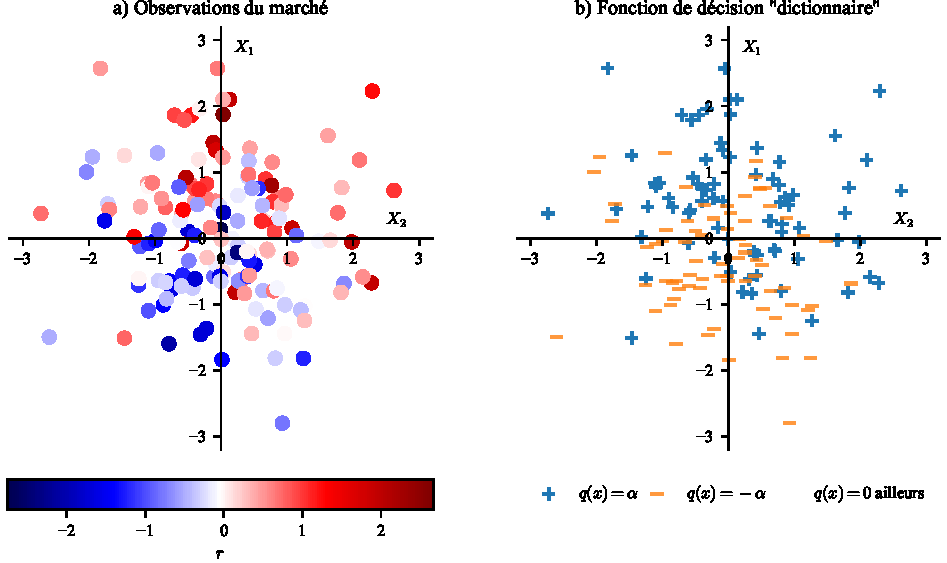
\includegraphics[width=\textwidth]{../experiments/fig/demo_1.pdf}
  \caption[Décision dictionnaire]{Illustration d'une fonction de décision ``dictionnaire''
    dont le risque de généralisation est arbitrairement élevé. Le marché est ici constitué
    de deux variables $X_1$ et $X_2$ (l'abscisse et l'ordonnée des deux figures). Le
    panneau a) présente un ensemble d'entraînement $\S_n$ $(n=150)$ où le gradient de
    couleur indique l'intensité du rendement associé à chaque observation. Le panneau b)
    présente la fonction de décision ``dictionnaire'' construite à partir de
    $\S_n$. L'investissement préconisé par $q$ suite à une observation $x\in\X$ sera nul si
    $x$ ne figure pas dans l'ensemble d'entraînement, mais sera positif ($+\alpha$) si son
    rendement associé est positif et négatif ($-\alpha$) dans le cas contraire. L'utilité
    espérée en échantillon $\hEU(q)$ est arbitrairement élevée à mesure que
    $\alpha\to\infty$, mais si $\X$ est dense dans $\Re^2$, alors $\EU(q) = u(0)$. Le risque de
    généralisation de la décision $q$ est donc à son tour arbitrairement élevé.}
  \label{fig_demo1}
\end{figure}

On peut alors faire appel au principe du \textit{rasoir d'Occam} pour éviter que des
fonctions de décision comme celle-ci ne soient favorisées. Ce principe suggère en effet
qu'une hypothèse trop complexe devrait être découragée au profit d'une hypothèse plus
simple (voir \cite{vapnik1998statistical} pour une discussion approfondie). Intuitivement,
si $\mathscr{C}(q) \in \Re$ permettait de mesurer la complexité d'une fonction de décision
$q$, on pourrait \textit{régulariser} l'objectif pour que l'investisseur cherche plutôt à
\begin{equation}
  \maximizeEquation{\hEU(q) - \lambda\mathscr{C}(q).}
\end{equation}
Différentes valeurs de $\lambda$ favorisent alors des solutions plus ou moins complexes. En
utilisant une technique de \textit{validation croisée}, il y a alors moyen de déterminer
le niveau de complexité permettant de minimiser le risque de généralisation.

On verra en outre aux Sections \ref{sec:algap} et \ref{sec:bound} qu'il existe pour
certaines classes de fonctions de décision une mesure de complexité particulière qui
permet d'établir des garanties statistiques sur le risque de généralisation. 

\paragraph{Risque in-échantillon et hors échantillon}

 une telle fonction $q$ est qu'elle se généralise très mal. En effet
pour toute observation $x$ qui ne figurerait dans l'ensemble d'entraînement, $q$
prescrirait alors un investissement nul. Il y a alors une énorme différence entre
l'utilité observée au sein de notre échantillon et l'utilité hors échantillon.

Donnée une fonction de décision $q \in \Q$ et un échantillon de $M$, on définit le
\textit{risque in-échantillon} ou \textit{risque empirique} par
\begin{equation}
  \hat R(q) = n^{-1}\sumi \ell(r_i\,q(x_i)),
\end{equation}
où $\ell = -u$. De la même façon, on définit le \textit{risque hors-échantillon} ou
\textit{erreur de généralisation} par
\begin{equation}
  R(q) = \E \ell(R \cdot q(X)).
\end{equation}
On peut souhaiter d'une bonne fonction de décision qu'elle performe bien hors échantillon,
aussi la quantité $R(q) - \hat R(q)$ sera-t-elle primordiale et beaucoup d'attention lui
sera consacrée dans les prochaines sections. Notons que le risque hors-échantillon étant
théoriquement impossible à calculer, en pratique on segmentera l'ensemble d'échantillonage
en deux parties, l'une dédiée à l'apprentissage, l'autre à évaluer la performance hors
échantillon.


\paragraph{Régularisation}

Afin de contrecarrer le risque hors échantillon, la solution est en fait de pénaliser la
complexité de la fonction de décision $q$ (rasoir d'Occam). Ainsi, on étudiera en
profondeur le choix d'une fonctionelle $R : Q \to \Re$ permettant de quantifier la complexité
de $q$. L'objectif serait alors
\begin{equation}
  \maximizeEquation[q \in \Q]{n^{-1} \sumi u(r_i\, q(x_i)) - R(q).}
\end{equation}
Par exemple, comme les mesures sur $x$ peuvent comporter de l'incertitude ou du bruit, il
serait souhaitable que la décision $q(x_1)$ soit proche de $q(x_2)$, si $x_1$ et $x_2$
sont eux même proches dans l'espace $\X$. Si $R$ encodait une telle préférence, ne
fonction discontinue comme le dictionnaire présenté plus haut sera alors hautement
défavorisée, et une fonction plus lisse y serait préférée.

\todo{Introduire la validation croisée ainsi que le paramètre $\lambda$ dans l'objectif.}



\paragraph{Espaces de décision}

En pratique, ce mémoire ne considérera que des espaces de Hilbert pour $\Q$. Un des
avantages des espaces de Hilbert, c'est qu'ils induisent naturellement une notion de norme
$\|\cdot\|_H$, qu'on peut intuitivement relié au concept de complexité. Nous nous
intéresserons donc aux propriétés induites par $R(q) = \|q\|_H^2 = \langle q, q \rangle$. Il y a
aussi moyen, sous des conditions assez techniques (théorème de la représentation) de
généraliser la norme $L_2$ de $q$ à une norme $L_p$ général. En particulier, nous verrons
qu'une régularisation donnée par norme $L_1$ induit certaines propriétés d'éparsité dans
la solution.


\paragraph{Décisions linéaires}

De façon générale, la forme de décision la plus simple est celle qui combine linéairement
les $p$ observations de $x \in \X \subseteq \Re^p$; autrement dit lorsque qu'on contraint
$\Q = \X^*$, \ie, à l'espace dual de $\X$. En langage plus clair, à toute fonction
$q \in \Q$ il existe un vecteur de dimension $p$ tel que la décision dérivée de
l'observation $x$ sera donnée par $q(x) = \langle q, x \rangle = q^Tx$.

La régularisation $L_2$ de $q$ devient alors tout simplement $R(q) = q^Tq = \|q\|^2$ et la
fonction optimale de décision $q^\star$ sera alors déterminée en résolvant le problème
d'optimisation suivant:
\begin{equation}
  \maximizeEquation[q \in \Re^p]{n^{-1}\sumi u(r_i\,q^Tx_i) - \lambda \|q\|^2.}
\end{equation}



\subsection{Dimensionalité de l'information}

\todo{Discussion du phénomène big data, de l'importance de $p$}



\subsection{Risque et garanties statistiques sur la décision}
\todo{Discussion sur les méthodes de risques hors échantillon, complexité de
  l'échantillonage, mesure Rademacher, distance par rapport à la ``meilleure'' décision}



\subsection{Interprétations}

\paragraph{Interprétation géométrique dans l'espace $X$}

\paragraph{Interprétation statistique (avec matrix covariance)}

\par\paragraph{Autre?}



\subsection{Objectifs et contributions}

Ce mémoire cherche donc à dégager les principales caractéristiques de cet algorithme
d'apprentissage appliqué à la gestion de portefeuille. Les contributions apportées sont
nombreuses.

D'abord, et c'est son but, cette méthode est parfaitement adaptée pour tenir en compte des
informations de marché dont la valeur ajoutée est \textit{a priori} inconnue. Une analyse
de covariance entre ces variables d'information et les réalisations du rendement permet
naturellement d'en avoir une certaine idée, mais une telle analyse ne tient pas compte de
l'utilité de l'investisseur et n'est pas régularisée. De plus une simple analyse en
covariance présuppose une dépendance \textit{linéaire} entre les rendements et les
variables de marché. La méthode par noyaux proposée à la Section \ref{sec:algap} offre au
contraire une richesse supplémentaire au modèle permettant d'exprimer des situations non
linéaires.

En fait, le faible nombre d'hypothèses sur la loi de marché (voir Section \ref{sec:bound})
permet à ce modèle de s'éloigner radicalement de l'approche courament employée en
tarification d'instruments financiers où les rendements sont modélisés selon une
distribution particulière: on peut penser par exemple à l'exemple classique du modèle
Black Scholes où le rendement est donné par une simple loi normale (voir
\cite{shreve2004stochastic}), ou à des modèles plus sophistiqués de tarification d'option
qui inclueraient des processus à saut (voir par exmeple \cite{madan1998variance}.

De plus, ce modèle est d'une grande flexibilté puisqu'il accepte toute forme d'utilité
monotone concave et fournit à l'investisseur des garanties probablisites exprimées en
rendement équivalent sur les erreurs de généralisation et de sous optimalité encourues. En
fait, non seulement ces erreurs sont connues, mais leurs ordres de convergence le sont
elles aussi. Ainsi, un investissseur est en mesure de prédire de combien peut décroître ou
augmenter l'erreur maximale hors échantillon lorsque de nouveaux échantillons ou de
nouvelles variables de marché sont ajoutés pour la prise de décision.

Notons par ailleurs que ce mémoire a aussi le mérite de s'inscrire dans la recherche en
apprentissage statistique en explorant de nouvelles formes de fonction de perte. Deux
classes de problèmes sont traditionnellement considérées : la régression et la
classification. Or, d'une certaine façon, notre problème emprunte des éléments propres à
ces deux classes de problèmes. D'abord avec la régression puisqu'on cherche dans les deux
cas à obtenir une quantité scalaire. Notre problème en diffère toutefois puisque,
contrairement à la régression où on cherche à \textit{minimiser} la distance entre un
estimateur et les données du problème, l'algorithme d'investissement proposé ici cherche
plutôt à \textit{amplifier} (positivement ou négativement selon le cas) les valeurs (les
rendements) du problème. 

On se rapproche également des problèmes de classification puisque leur objectif (non
régularisé) y sont de la forme
\begin{equation}
  \minimizeEquation[q]{n^{-1}\sumi\ell(y_i\,q^Tx_i)}
\end{equation}
où $y_i\in\{-1,+1\}$ est la cible du problème et $\ell:\Re\to\Re$ mesure l'adéquation entre
$y_i$ et $q^Tx_i$. Typiquement $\ell(z)$ est nul lorsque $z\ge0$, \ie\ lorsque $y_i$ et
$q^Tx_i$ sont du même signe, et est positif (constant ou croissant) dans la région où
$z<0$, \ie\ lorsque $y_i$ et $q^Tx_i$ sont de signes opposés. En fait, la théorie des
machines à vecteurs de support est un cas particulier de notre problème d'optimisation
d'utilité lorsqu'on ne considère que le signe des rendements et qu'on emploie une fonction
d'utilité $u$ nulle sur l'intervalle $[1,\infty]$. Voir \cite{mohri2012foundations} pour une
introduction générale aux problèmes de régression et de classification.

Finalement, ce travail apporte également une modeste contribution au domaine des
statistiques multivariées puisqu'une façon de concevoir le problème de maximisation
d'utilité est comme celui des périls inhérents à l'estimation d'un \textit{vecteur} de
covariance non centrée entre une variable aléatoire scalaire et un vecteur aléatoire. En
effet, dans le cas limite où l'utilité est neutre au risque, \ie\ $u(x) = x$, le problème
de maximisation d'utilité revient à
\begin{equation}
  \maximizeEquation[q]{\E(R\,q^TX) - \tfrac{\lambda}{2}\|q\|^2,}
\end{equation}
dont la solution est donnée par $q =  \lambda^{-1}\E(RX)$, \ie\ la covariance non centrée
entre $R$ et $X$. Ainsi, tous les résultats dérivés dans ce travail s'appliquent aussi à
ce problème d'estimation statistique.



%%% Local Variables:
%%% mode: latex
%%% TeX-master: "memoire"
%%% End:
